

\subsection{Cross Sections as a function of muon momentum}
%Results in P$_\mu$ 

The differential cross section as a function of P$_\mu$ for interactions on the CH, C, H$_{2}$O, Fe, and Pb targets, respectively, are shown in Fig.~\ref{figure:xsec_muon_p}. P$_\mu$ is the muon momentum in GeV/c.  The uncertainties broken down by source for both the absolute cross sections and the cross section ratios as a function of P$_\mu$ can be found in Fig.~\ref{fig:xsec_err_muon_p}.
Qualitatively, the MINERvA tune does a fairly good job describing the data.  The main area of disagreement is in the interactions on Pb where the data has a bit higher cross section in the peak region of P$_\mu$.

% tki_muon_p xsecs
\begin{figure}[h]  
	\centering
  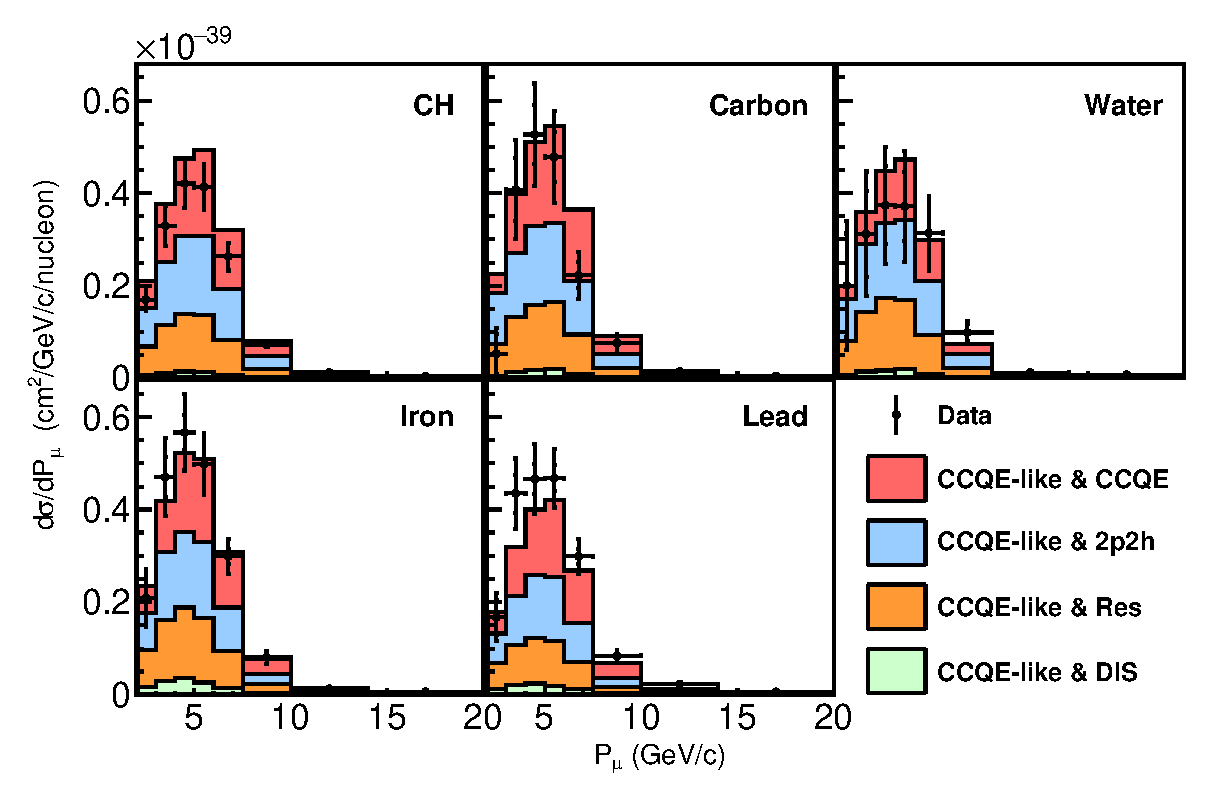
\includegraphics[width=\linewidth]{Figures/xsec_five_square/muon_p.eps}
	\caption{The differential cross section as a function of P$_\mu$ for CH, C, H$_{2}$O, Fe, and Pb targets, along with the predictions for the different quasielastic-like signal processes.}
	\label{figure:xsec_muon_p}
\end{figure}



The differential cross section as a function of P$_\mu$ for the different targets as compared to a range of models is given in Fig.~\ref{fig:models_muon_p}. The qualitative features of the data are exhibited by the  models.  NEUT gives a higher cross section than is seen in the data, particularly for the larger targets.  The hN versions of GENIE also show this behavior in in Pb.
The \chisq\ between the cross sections and the models can be found in Table~\ref{tab:muonmomentum}.

% comparisons to generators muon_p
\begin{figure}
    \centering
        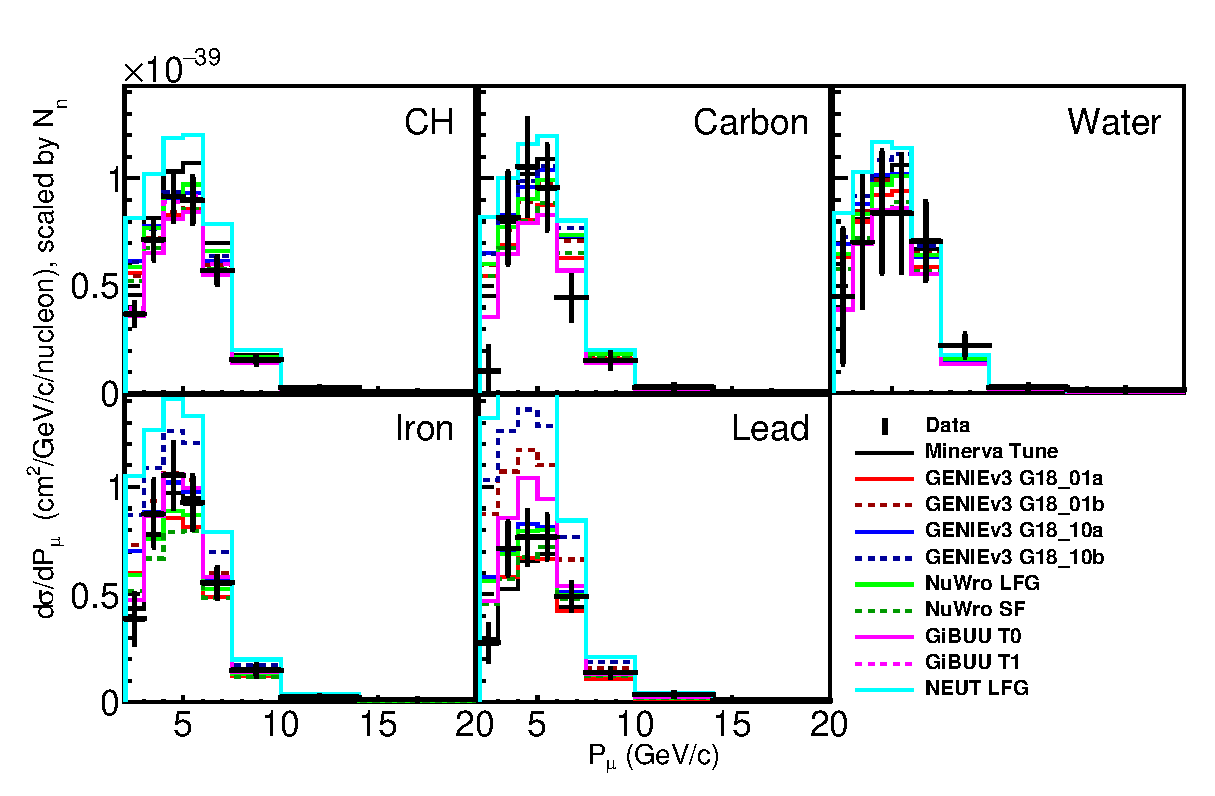
\includegraphics[width=\linewidth]{Figures/gencompare/muon_p_5square.eps}
    \caption{Cross section measurements and predictions as a function of P$_\mu$ for different targets and for a selection of different generator and model choices.}
    \label{fig:models_muon_p}
\end{figure}

The ratio of the differential cross section as a function of  P$_\mu$ for each nuclear target (C, H$_{2}$O, Fe, Pb) to that for scintillator is shown in 
Fig.~\ref{Figure:Gencompare_pmu_ratio}. Generally, the models cover the data reasonably well for the three smaller targets. For the Pb target, the ratio for the MINERvA tune is significantly lower than the data and the predictions from the other models.  Also on Pb, at lower P$_\mu$ the hN versions of GENIE and NEUT and GiBUU all exhibit higher ratios than seen in the data.
The \chisq\ between the cross section ratios and the models can be found in Table~\ref{tab:muonmomentum}.

\begin{figure}
    \centering            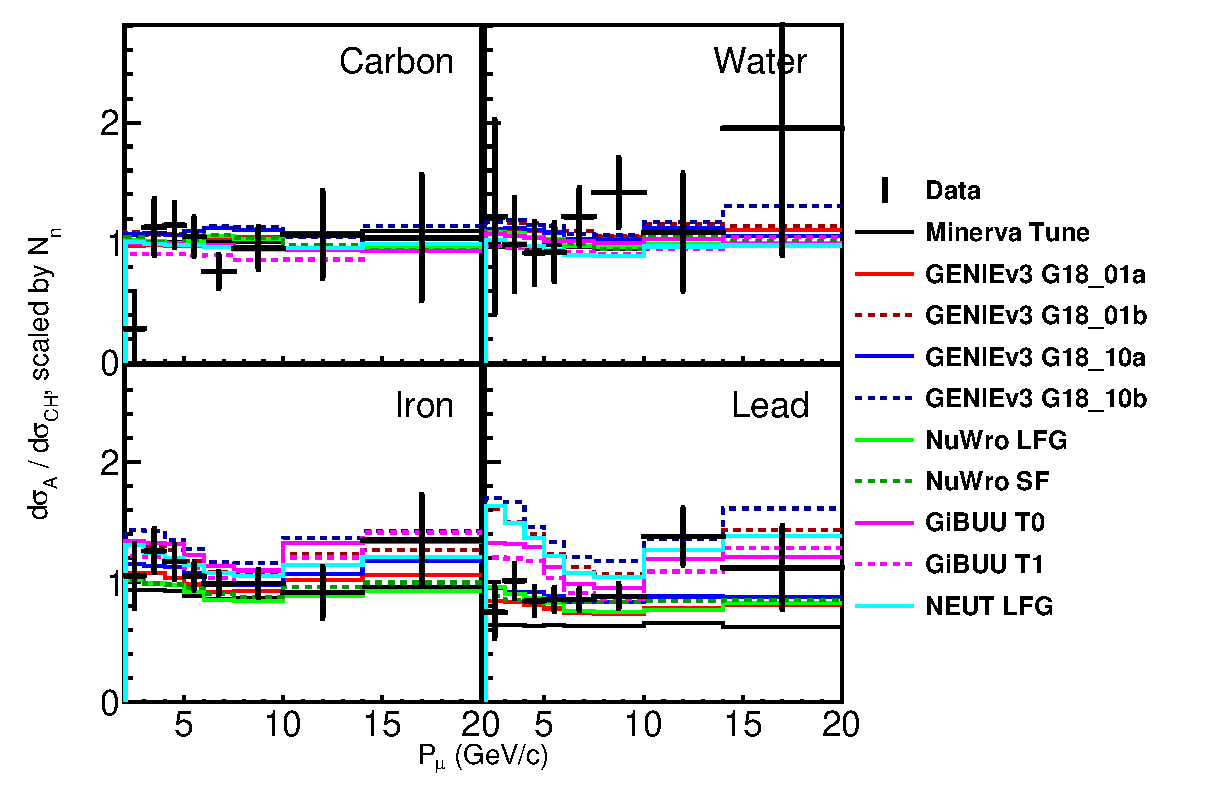
\includegraphics[width=\linewidth]{Figures/gencompare/muon_p_4square.eps}
    \caption{$P_\mu$ cross-section ratio generator comparison for multiple targets.  Changes to the FSI model (GENIE ``a'' to ``b'') in GENIE change the cross section ratio more than changes to the 2p2h model (GiBUU T0 to GiBUU T1) or changes to the initial state (GENIE 1 to GENIE 10) or (NuWro LFG to NuWro SF).  The changes to the ratio are significant across all muon momenta, unlike in other kinematic variables.}
        \label{Figure:Gencompare_pmu_ratio}
\end{figure}
